\subsection{Dialogue Act Modeling for Automatic Tagging and Recognition of Conversational Speech \cite{Stolcke2000}}

This paper describes a statistical approach for modeling \emph{dialogue acts (DAs)} on conversational speech, i.e., speech-act-like units such as \emph{Statement}, \emph{Question}, \emph{Backchannel}, etc. The proposed model detects and predicts dialogue acts based on lexical, collocational, and prosodic cues, as well as on the discourse coherence. It develops a probabilistic integration of speech recognition with dialogue modeling, to improve both speech recognition and dialogue act classification accuracy.

The goal of this paper is twofold: 1) presets a comprehensive framework for modeling and automatic classification of DAs, and proposes a framework that provides a mathematically principled way to condition the speech recognizer on conversation context through dialogue structure; 2) presents results obtained with this approach on a large, widely available corpus of spontaneous conversational speech.

This paper follows a recent standard for shallow discourse structure annotation, the \emph{Dialogue Act Markup in Several Layers (DAMSL)} tag set, which aims to provide a domain-independent framework for dialogue annotation.

The mathematical and computational framework used in the paper is the \emph{hidden Markov model (HMM)}. Given all available evidence $E$ about a conversation, the goal is to find the DA sequence $U$ that has the highest posterior probability $P(U|E)$ given that evidence.
$$U^* = \arg\max_U P(U|E) = \arg\max_U P(U) P(E|U).$$
Next we will discuss the prior probability $P(U)$, and the posterior probability $P(E|U)$ respectively.

In modelling the prior distribution $P(U)$, the paper assumes that the distribution is Markovian, i.e., each $U_i$ depends only on a fixed number $k$ of preceding DA labels:
$$P(U_i | U_1, ..., U_{i-1}) = P(U_i | U_{i-k}, ..., U_{i-1}).$$
The paper trains standard backoff N-gram models, using the frequency smoothing approach. The authors also tried several alternative approaches, but there was no significant improvement over the simple N-gram method.

The computation of $P(E|U)$ depends on the types of evidence use. The paper used the following three types of sources of evidence, either alone or in combination:
\begin{itemize}
\item{\textbf{Transcribed words}\\
$P(W|U)$, where $W$ refers to the true (hand-transcribed) words spoken in a conversation.
}
\item{\textbf{Recognized words}\\
A standard approach is to use the 1-best hypothesis. A more thorough approach is to compute $P(A|U)$ (where $A$ is the acoustics input) by decomposing it into an acoustic likelihood $P(A|W)$ and a word-based likelihood $P(W|U)$:
$$P(A|U) = \sum_W P(A|W) P(W|U).$$
}
\item{\textbf{Prosodic features}\\
$P(F|U)$, where $F$ are the features capturing various aspects of pitch, duration, energy, etc., of the speech signal. For the prosodic classifiers, the paper used CART-style decision trees. One example in the corpus was the distinction between backchannels and agreement. The prosodic tree trained on this task is shown in Figure \ref{fig:stolcke00-decision_tree}. The paper also tried to use neural network classifiers on this task, and tested
various network structures. However, there was no encouraging result.
\begin{figure}[h]
  \centering
  % Requires \usepackage{graphicx}
  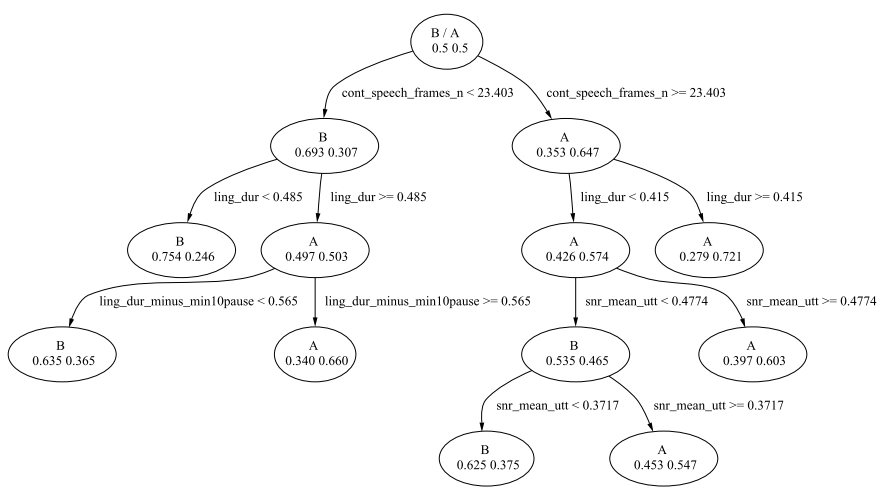
\includegraphics[width=\linewidth]{stolcke00-decision_tree.png}\\
  \caption{Decision tree for the classification of backchannels and agreements.}\label{fig:stolcke00-decision_tree}
\end{figure}
}
\end{itemize}

The paper proposes a method to combine multiple knowledge source, by using the following approximation:
\begin{align*}
P(A_i, W_i, F_i | U_i) &= P(A_i, W_i | U_i) P(F_i | A_i, W_i, U_i)\\
                       &\approx P(A_i, W_i | U_i) P(F_i | U_i).
\end{align*}

The HMM representation allows using efficient dynamic programming algorithms to compute relevant aspects of the model, such as: 1) the most probable DA sequence (the \emph{Viterbi algorithm}); 2) the posterior probability of various DAs for a given utterance (the \emph{forward-backward algorithm}).

The paper considers ways to use DA modeling to enhance automatic speech recognition (ASR). The first method is called \emph{mixture-of posteriors}, which yields:
$$P(W_i | A_i, E) = \sum_{U_i} \frac{P(W_i | U_i) P(A_i | W_i)}{P(A_i | U_i)} P(U_i | E).$$
The second method, called \emph{mixture-of-LM}, results in:
$$P(W_i | A_i, E) \approx (\sum_{U_i} P(W_i | U_i) P(U_i|E)) \frac{P(A_i |W_i)}{P(A_i)}.$$

The experiments confirmed that DA modeling can improve word recognition accuracy quite substantially in principle, at least for certain DA types.But the skewed distribution of DAs limits the usefulness of the approach on the Switchboard corpus. The paper suggests that the benefits of DA modeling might be more pronounced on corpora with more even DA distribution, which is typically the case for task-oriented dialogues.
